\documentclass[preprint,11pt]{elsarticle} % Main formatting of the paper

% Page Layout and Formatting
\usepackage[margin=2.5cm]{geometry} % Set page margins
\usepackage{lineno} % For line numbers in the document
\usepackage{titlesec} % Control section title formatting
% Referencing and Hyperlinks
\usepackage{hyperref} % Create hyperlinks in the document (for references, citations, tables, etc.)

% Mathematics and Theorem Environments
\usepackage{amsmath} % Provides enhanced math typesetting (equations, symbols)
\usepackage{amsfonts} % Additional fonts for math (e.g., Blackboard bold, Fraktur)
\usepackage{amsthm} % For defining theorem-like environments (theorems, propositions, definitions)
\newtheorem{definition}{Definition} % Define the environment for definitions
\newtheorem{proposition}{Proposition} % Define the environment for propositions

% Figures and Tables
\usepackage{graphicx} % Insert images and figures
\usepackage{subcaption} % Create subfigures under a single figure environment
\usepackage{wrapfig} % Allows text to wrap around figures
\usepackage{float} % Control figure and table placement (for [H] option)
\usepackage{slashbox} % Create diagonal slash tables (used for splitting cells)

\bibliographystyle{ieeetr}  % Specifies the IEEE Transactions reference style

% Custom commands
\titleformat{\subsection}
  {\normalfont\bfseries} % Format for subsection title
  {\thesubsection}{1em}{} % Format for subsection number and title
 % Include file for custom LaTeX commands

%%%%%%%%%%%%%%%%---Main Document Starts---%%%%%%%%%%%%%%%%
%%%%%%%%%%%%%%%%%%%%%%%%%%%%%%%%%%%%%%%%%%%%%%%%%%%%%%%%%%

\begin{document}


\begin{frontmatter}

\title{
\hrule height 2.5pt
\vskip 15pt
\textbf{Multiagent Q-learning with Sub-Team
Coordination}
\vskip 10pt
\hrule height .8pt
}

% \title{Multiagent Q-learning with Sub-Team}

\author[1]{Wenhan Huang\corref{cor1}}
\author[2]{Kai Li}
\author[2]{Kun Shao}
\author[3]{Tianze Zhou}
\author[4,5]{Matthew E. Taylor}
\author[2]{Jun Luo}
\author[6]{Dongge Wang}
\author[2]{Hangyu Mao}
\author[2,7]{Jianye Hao}
\author[8]{Jun Wang}
\author[9]{Xiaotie Deng\corref{cor2}}

\cortext[cor1]{This work was done when Wenhan Huang was an intern at Huawei Noah’s Ark Lab.}
\cortext[cor2]{Corresponding author}

\address[1]{Shanghai Jiao Tong University}
\address[2]{Huawei Noah's Ark Lab}
\address[3]{Beijing Institute of Technology}
\address[4]{University of Alberta}
\address[5]{Alberta Machine Intelligence Institute (Amii)}
\address[6]{EPFL}
\address[7]{Tianjin University}
\address[8]{University College London}
\address[9]{Peking University}

\ead{rowdark@sjtu.edu.cn}
\ead{likai210@huawei.com}
\ead{shaokun2@huawei.com}
\ead{jun.luo1@huawei.com}
\ead{maohangyu1@huawei.com}
\ead{simsimizt@126.com}
\ead{matthew.e.taylor@ualberta.ca}
\ead{dongge.wang@epfl.ch}
\ead{jianye.hao@tju.edu.cn}
\ead{jun.wang@cs.ucl.ac.uk}
\ead{xiaotie@pku.edu.cn}


\begin{abstract}
In many real-world cooperative multiagent reinforcement learning (MARL) tasks, teams of agents can rehearse together before deployment, but then communication constraints may force individual agents to execute independently when deployed. Centralized training and decentralized execution (CTDE) is increasingly popular in recent years, focusing mainly on this setting. In the value-based MARL branch, credit assignment mechanism is typically used to factorize the team reward into each individual’s reward — individual-global-max (IGM) is a condition on the factorization ensuring that agents’ called \emph{multiagent Q-learning with sub-team coordination }(QSCAN), to flexibly represent sub-team coordination while honoring the IGM condition. QSCAN encompasses the full spectrum of sub-team coordination according to sub-team size, ranging from the monotonic value function class to the entire IGM function class, with familiar methods such as QMIX and QPLEX located at the respective extremes of the spectrum. Experimental results show that QSCAN’s performance dominates state-of-the-art methods in matrix games, predator-prey tasks, the Switch challenge in MA-Gym. Additionally, QSCAN achieves comparable performance to those methods on the StarCraft multiagent benchmark.
\end{abstract}

\end{frontmatter}

\section{\textbf{Introduction}}
    In many real-world cooperative multiagent reinforcement learning (MARL) tasks, agents can train together but must execute independently due to communication constraints. The Centralized Training and Decentralized Execution (CTDE) framework is popular in this context, focusing on training agents as a team but executing individually. This approach leverages the benefits of centralized training, such as improved coordination and learning efficiency, while maintaining the flexibility and scalability of decentralized execution. The introduction section highlights the importance of balancing these aspects to achieve effective and practical MARL solutions. It also emphasizes the challenges and potential strategies for optimizing agent performance in such settings.


\section{Background}
    \textbf{Dec-POMDP.} We characterize a fully cooperative multiagent learning task as a \emph{decentralized partially observable Markov decision process} (Dec-POMDP) with a tuple $\mathcal{M} = \langle\mathcal{N}, \mathcal{S}, \mathcal{A}, T, \Omega, O, \Gamma, \gamma \rangle$ \cite{r1}. Here, $\mathcal{N} = \{1,2,\ldots, n\}$ is a set of agents, and $\mathcal{S}$ is a set consisting of environment states. At each time step, each agent $i \in \mathcal{N}$ chooses an action $a_i \in \mathcal{A}_i$, forming a joint action $a \in \mathcal{A} = \prod_{i=1}^n \mathcal{A}_i$ of all agents. This leads to a transition from the current state $s$ to the next state $s'$ governed by a transition function $T(s' \mid s, a)$. Due to the partial observability, $\Omega = \prod_{i=1}^n \Omega_i$ is the joint observation set, where $\Omega_i$ is the partial observation set of agent $i$. $O(o \mid s, a')$ is the conditional probability of joint observations given the current state $s$ and the previous joint action $a'$. $r: \mathcal{S} \times \mathcal{A} \rightarrow \mathbb{R}$ denotes the global reward function. The objective of the task is to maximize the total discounted reward $\sum_{t=0}^\infty \gamma^t r(s_t, a_t)$ where $\gamma \in [0, 1)$ is a discount factor, $s_t$ and $a_t$ are the state and the joint action at time step $t$, respectively.

    \textbf{Multiagent deep Q-learning.} For a given joint policy $\pi$ of agents, let the global action-value function $Q^\pi(s_t,a_t)=\mathbb{E}[\sum_{k=0}^\infty \gamma^i r(s_{t+k},a_{t+k})]$ denote the expected discounted reward starting at state $s_t$ with joint action $a_t$. When $\pi$ is optimal, the global action-value function satisfies the Bellman optimality equation. Due to the partial observation setting, we use the joint observation history in place of the state $s$. Multiagent deep Q-learning represents the global action-value function $Q_{\text{tot}}$ with a deep neural network parameterized by $\theta$. In centralized algorithms, the parameters are obtained by minimizing the expected TD error $\mathcal{L}= \mathbb{E} \left[ \left( r + \max_{a'} Q_{\text{tot}}(s', a'; \theta^-) - Q_{\text{tot}}(s, a; \theta) \right)^2 \right]$, where $\theta^-$ is the parameter of a target network.
    
    \textbf{Value-based methods in the CTDE paradigm.} A typical dilemma in cooperative multiagent learning is that each agent should act independently based on its observation, but global information is needed to make a good decision for teamwork. CTDE \cite{r2} is the popular framework in recent years to remedy this challenge. In most value-based methods in the CTDE paradigm, the individual action-value functions for all players are trained in a centralized way, and an agent only relies on its trained individual function and its partial observation to choose actions. Due to the partial observation, \cite{r3} suggests that the optimal joint strategy should be executed as each agent plays its own optimal strategy concurrently. Formally, the condition of such action-value functions can be described as follows:

    % In your document body:
    \begin{definition}[Individual-Global-Max (IGM) \cite{r4}]
        For a global action-value function $Q_{tot} : \mathcal{T} \times \mathcal{A} \to \mathbb{R}$ and a series of individual action-value functions $[Q_i]_{i=1}^n$ with $Q_i : \mathcal{T}_i \times \mathcal{A}_i \to \mathbb{R}$, where $\tau \in \mathcal{T}$ is the joint history and $\tau_i \in \mathcal{T}_i$ is agent $i$'s individual history, if $\forall \tau \in \mathcal{T}$
        \[
            \left(\arg\max_{a_1 \in \mathcal{A}_1} Q_1(\tau_1,a_1),\ldots, \arg\max_{a_n\in \mathcal{A}_n} Q_n(\tau_n,a_n)\right) \in \arg\max_{a \in \mathcal{A}} Q_{tot}(\tau,a),
        \]
        then we say that $[Q_i]_{i=1}^n$ satisfy the IGM condition for $Q_{tot}$.
    \end{definition}

    Once a framework satisfies the IGM condition, the global action value can be maximized efficiently via individually optimal choices of all the agents.

    \textbf{Self-attention mechanism.} 
    The self-attention mechanism \cite{r5} is widely used to extract the relationship between different positions of an input sequence in the natural language processing community. It can efficiently relate its different inputs. In the MARL community, the self-attention mechanism is used to learn the relationship between a team of agents. Jiang and Lu \cite{r6} employ the self-attention mechanism to learn the communication among agents. Li et al. \cite{r7} use the self-attention mechanism to determine the implicit coordination graph structure of agents. The formula of the self-attention mechanism can be written as:$
    \text{Attention}(\mathcal{Q}, \mathcal{K}, \mathcal{V}) = \text{softmax}(\mathcal{Q}\mathcal{K}^T)\mathcal{V},
    $where $\mathcal{Q}$, $\mathcal{K}$, and $\mathcal{V}$ denote the query vectors, the key vectors, and the value vectors, respectively. The weight of each value $\mathcal{V}_j$ to the $i$-th output is computed by the compatibility $\mathcal{Q}_i\mathcal{K}_j$, a dot product of the $i$-th query vector and $j$-th key vector. The softmax activation function translates the dot product into a measurement of attention.
    

\section{Sub-TeamCoordination Patterns}
\label{sec:Sub-TeamCoordination Patterns}
    In a large multiagent system, the task is usually decomposed as several sub-tasks so that agents can accomplish each sub-task separately. For each sub-task, a sub-team is formed with several agents.Besides, one agent could simultaneously belong to different sub-teams. This sub-team organization is general and can implicitly characterize most coordination patterns among agents \cite{r8}. In this paper,we exploit sub-team coordination patterns in value factorization frameworks.To this end, we would first explore sub-team coordination patterns in this section and then discuss the concrete architectures in the next one.    


    \begin{proposition}
        Consider a fixed mixing function $f : \mathbb{R}^{n} \times \mathcal{S} \to \mathbb{R}$. If $Q_{tot}(s, \cdot) = f(Q_1, \ldots, Q_n, s)$, where $Q_{tot}$ and $[Q_i]_{i=1}^n$ satisfy the IGM condition consistently for any function $Q_i(s, \cdot)$ which contains a unique maximum point, then $f$ should satisfy $\forall i \forall x_i \in \mathbb{R}, \frac{\partial f(x_1,\ldots,x_n,s)}{\partial x_i} \geq 0$.
    \end{proposition}

    \textbf{The grand team.} Only considering the grand team $\{1,\ldots,n\}$ is another typical solution. In this factorization, we can assume $Q_{\{1,\ldots,n\}} = Q_{tot}$. With the individual action values $\{Q_i\}$, the global action value can be written as $Q_{tot}(s,a) = f(Q_1,\ldots,Q_n,s,a)$. This kind of value factorization may not always satisfy the IGM condition.

    \begin{wrapfigure}{r}{0.3\textwidth}
    \centering
    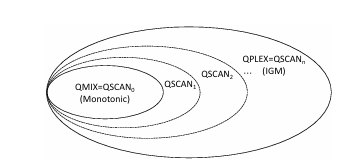
\includegraphics[width=\linewidth]{images/ima3.png}
    \caption{Coordination hierarchy. We identify and prove a general representation of relation among sub-team coordination function classes, from the monotonic function class to the IGM function class.}
    \label{fig:ima3}
    \end{wrapfigure}

    
    QPLEX \cite{r8}, an instance of this function class, employs the duplex dueling structure and transfers the IGM condition to advantage values $A(s, \mathbf{a}) = Q(s, \mathbf{a}) - V(s)$, where $V(s) = \max_{\mathbf{a}} Q(s, \mathbf{a})$. The global advantage value $A_{\text{tot}}$ is factorized as:$A_{\text{tot}}(s, \mathbf{a}) = \sum_{i=1}^n \lambda_i(s, \mathbf{a}) A_i(s, a_i),$where $[\lambda_i(s, \mathbf{a})]_{i=1}^n$ is an importance weight. The joint action $\mathbf{a}$ here is considered atomic. As pointed in \cite{r8}, the IGM function space is equivalent to the space that QPLEX can represent. However, the indivisibility of the joint action $\mathbf{a}$ in the grand team may prevent the mixing network from reusing the knowledge from previous coordination patterns, leading to poor generalization. Specifically, the importance weights using atomic joint actions in QPLEX may not perform well in credit assignment when the correlations among agents become complicated.As the predator-prey results shown in \cite{r9} and \cite{r8}, QPLEX requires additional tuning of the exploration rate to extract predators’ coordination patterns.
    
        

\section{\textbf{Multiagent Q-learning with Sub-team Coordination}}
    In this section, we introduce the specific architecture of QSCAN, a value factorization framework that leverages sub-team coordination patterns while adhering to the IGM condition. We begin by outlining the base architecture, which utilizes duplex dueling structures \cite{r10} to ensure the IGM condition is satisfied. Following this, we delve into the critical component of QSCAN—the sub-team coordination module—that defines the team's organization and coordination patterns. Several function classes can be derived from the QSCAN framework. Finally, we explore the coordination module in detail and present two practical architectures for QSCAN.

    \textbf{Sub-team Coordination and QSCAN Framework}
    We analyze the design of the theoretical coordination module which characterizes coordination patterns within \emph{k}-member sub-teams and then propose the \large{QSCAN} framework .Intuitively, the team reward can be creadited to each sub-team and then to each individual . Consider a sub-team $ST$ containing \emph{k} agents and $a_{ST}$ is $ST$'s joint action . The contribution of $ST$ can be assigned to each member \emph{i} with an importance weight $g_{i}^{ST}$ evaluating \emph{i}'s contribution in $ ST$.

    % \begin{align}
    %     A_{tot}(\textbf{\tau}, \textbf{a}) 
    %     & \approx \sum_{ST:ST \subseteq\mathcal{N},|ST|=k} \left[ \sum_{i \in ST} \left( g_i^{ST}(\tau, a_{ST}) \cdot A_i(\tau, a_i) \right) \right]\nonumber\\
    %     & = \sum_{i=1}^{n} \left( \sum_{ST: i \in ST \subseteq\mathcal{N}, |ST| = k} g_i^{ST}(\tau, a_{ST}) \right) A_i(\tau, a_i).\nonumber\\
    % \end{align}
    % Based on this factorization, ,we propose \large{$QSCAN_{\emph{k}}$}

    \begin{align}
        A_{tot}(\mathbf{\tau}, \mathbf{a})
        & \approx \sum_{\mathbf{ST} : \mathbf{ST} \subseteq \mathcal{N}, |\mathbf{ST}| = k}
        \left( \sum_{i \in \mathbf{ST}} \left( g_i^{\mathbf{ST}}(\mathbf{\tau}, \mathbf{a}_{\mathbf{ST}})
        \cdot A_i(\mathbf{\tau}, \mathbf{a}_i) \right) \right) \nonumber \\
        & = \sum_{i=1}^{n} \left( \sum_{\mathbf{ST} : i \in \mathbf{ST}
        \subseteq \mathcal{N}, |\mathbf{ST}| = k} g_i^{\mathbf{ST}}(\mathbf{\tau}, \mathbf{a}_{\mathbf{ST}})
        \right) A_i(\mathbf{\tau}, \mathbf{a}_i). \nonumber
    \end{align}

    Based on this factorization, ,we propose \large{$QSCAN_{\emph{k}}$}


\section{\textbf{Emperical Results}}
    We compare QPAIR and QSCAN with state-of-the-art MARL approaches, QMIX and QPLEX, in various coordination tasks, including matrix games, predator-prey challenges \cite{r8}, the Switch task \cite{r6}, and the StarCraft Multi-Agent Challenge (SMAC) \cite{r7}. For a fair comparison, the implementation of QSCAN uses one attention layer, that is, with sub-teams of size 2. The learning curves are plotted with a smooth factor of 0.6 except the last point. The implementation detail and environment detail are in Appendix C. 


    \subsection{Matrix Game}
    \begin{wraptable}{r}{.7\textwidth}
        \caption{Payoffs of a 3-player matrix game. Each player \emph{i} $\in$ \{ 1,2,3 \} has two actions \{ A,B \}.The complete payoff matrix is split into two submatrices according to player 1’s action a1.}
        \vspace{10pt}
        \begin{tabular}{cc}
             \begin{tabular}{c}
                 when $a_1=A$ \\[2ex]
                \begin{tabular}{|l||*{2}{c|}}\hline
                    \backslashbox{$a_{2}$}{$a_{3}$}
                    &\makebox[3em]{A}&\makebox[3em]{B}\\\hline\hline
                     A &0 &0\\\hline
                     B &\textbf{23}&12\\\hline
                \end{tabular}
             \end{tabular}
             &
             \begin{tabular}{c}
                 when $a_1=A$ \\[2ex]
                \begin{tabular}{|l||*{2}{c|}}\hline
                    \backslashbox{$a_{2}$}{$a_{3}$}
                    &\makebox[3em]{A}&\makebox[3em]{B}\\\hline\hline
                     A &17 &20\\\hline
                     B &03&17\\\hline
                \end{tabular}
             \end{tabular}
        \end{tabular}
        \label{tab:pay}
    \end{wraptable}

    Table ~\ref{tab:pay} shows the payoffs of a 3-player with 2-action matrix game. Fig ~\ref{fig:sub_learning_a} illustrates the empirical results for QMIX, QPLEX, QPAIR and QSCAN. Due to the relative overgeneralization,fails to find the optimal solution. QPLEX suffers another problem about the poor generalization. QSCAN and QPAIR can find the optimal solution more quickly because the pairwise coordination patterns provide more suitable generalization in this task. In the exploration period ,The pairwise coordination would allow the algorithm to explore the optimal solution more easily. Moreover, for all different random seeds in our experiments, QSCAN always finds the optimal solution rapidly in this matrix game.



    \begin{figure}[htbp]
        \centering
        \begin{subfigure}[b]{0.3\textwidth}
            \centering
            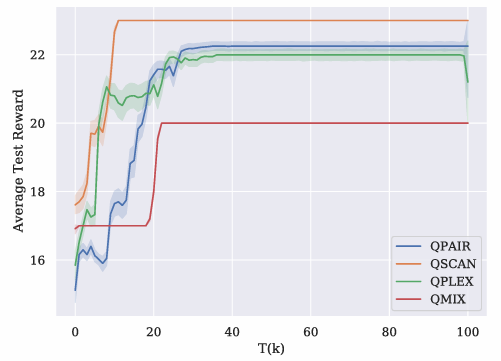
\includegraphics[width=\textwidth]{images/ima1.png}
            \caption{Matrix game.}
            \label{fig:sub_learning_a}
        \end{subfigure}
        \hfill
        \begin{subfigure}[b]{0.3\textwidth}
            \centering
            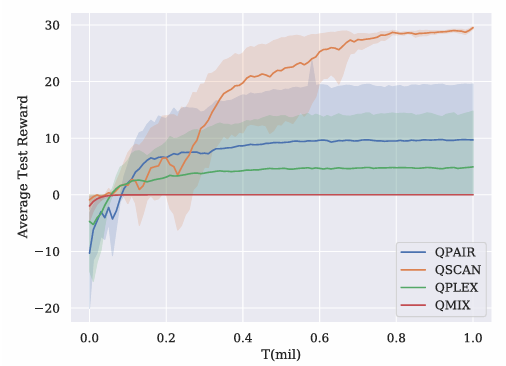
\includegraphics[width=\textwidth]{images/ima2.png}
            \caption{Predator-Prey (6 versus 6).}
            \label{fig:sub_learning_b}
        \end{subfigure}
        \hfill
        \begin{subfigure}[b]{0.3\textwidth}
            \centering
            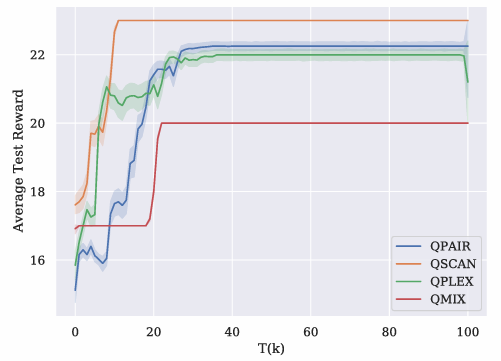
\includegraphics[width=\textwidth]{images/ima1.png}
            \caption{Switch4 challenge.}
            \label{fig:sub_learning_c}
        \end{subfigure}
        \caption{Learning curves of QPAIR, QSCAN, QPLEX, and QMIX in three different tasks. For the timestamp T, k and mil are short for 1s 'kilo' and 'million' respectively. The shaded area with 95\% confidence intervals is shown. Best viewed in color.}
        \label{fig:learning_curves}
    \end{figure}


    % \pagebreak

    \subsection{\large{TheStarCraft Multi-Agent Challenge}}

    \begin{wraptable}{r}{.6\textwidth}
        \caption{ Median of the test win rates in the SMAC.}
        \label{tab:tab2}
        \begin{tabular}{cccccc}
            \hline
            Scenario & QSCAN & QPAIR & QPLEX & QMIX \\
            \hline
            2s\_vs\_1sc & \textbf{100} & \textbf{100} & \textbf{100} & \textbf{100} \\
            2s3z & \textbf{100} & \textbf{100} & \textbf{100} & 97 \\
            3s5z & \textbf{98} & 97 & 97 & 94 \\
            1c3s5z & 88 & \textbf{97} & \textbf{97} & 94 \\
            2c\_vs\_64zg & 62 & 86 & \textbf{88} & 42 \\
            5m\_vs\_6m & \textbf{76} & 77 & 72 & 69 \\
            \hline
        \end{tabular}
    \end{wraptable}

    The StarCraft Multi-Agent Challenge (SMAC)\cite{r7} is a widely-used benchmark for cooperativeMARL.Weevaluate our approaches on a widerange of SMAC scenarios, including homogeneous (e.g., 5mvs6m) and heterogeneous (e.g.,3s5z) agents. Furthermore, we compare our approaches with state-of-the-art baselines: QMIX and QPLEX. The empirical results are shown in Table ~\ref{tab:tab2}, and the corresponding figures are presented in Appendix E.4.\\
    
        The results shows that \textbf{QSCAN} and \textbf{QPAIR} are superior to \textbf{QMIX} in most scenarios. QSCAN performs 
        almost well except for 2c\_vs\_64zg. Its win rate is about 20\% less than that of QPAIR or QPLEX. 
        2c\_vs\_64zg needs the coordination of two colossi, where the pairwise coordination characterized 
        by QPAIR coincides with the grand team coordination characterized by QPLEX. As QMIX does not 
        perform well in this scenario, we conjecture that this scenario requires the pairwise coordination 
        patterns rather than individual patterns. One possible reason for the performance of QSCAN could be 
        that the individual patterns through the residue links prevent QSCAN to achieve better performance in 
        this scenario. QPAIR achieves the best performance in some scenarios and no more than 2\% less 
        than the best one's win rate in other selected scenarios. Overall, our approaches achieve comparable 
        performances with the SOTA baseline QPLEX which uses the joint action in the mixing net.

\section{Conclusions and Future Work}

We propose QSCAN, a novel value-based multiagent reinforcement learning framework that can
characterize coordination patterns within sub-teams hierarchically and guarantee the IGM condition. QSCAN provides value factorization architectures with an expressive mixing network for the
centralized end-to-end training and learns a series of individual action-value functions for decentralized execution. We establish a coordination hierarchy based on QSCAN after analyzing the
sub-team factorization, and present two efficient implementations based on pairwise coordination
and self-attention mechanisms. Empirically, we show that our methods achieve better or comparable
performance with baselines in several benchmarks.

While our value-based architecture employs the duplex dueling structure for the sub-team factorization,
we believe that the sub-team factorization benefits other architectures, e.g., policy-based methods
like COMA \cite{r5}. As our discussion about sub-teams in Sec.~\ref{sec:Sub-TeamCoordination Patterns}, designing more effective hierarchical
structures for sub-team organization beyond the factorization on advantages, remains a challenge.
From theoretical side, it remains a problem about whether a general coordination hierarchy exists
according to the sub-team factorization $\frac{\partial Q_{tot}}{\partial Q_{ST}} \geq 0$ when sub-team size $k \geq \frac{n}{2}$. One more thing,
there has not been a universal organizational paradigm suitable for most tasks \cite{r9,r3}. Besides the
sub-team organization, exploring other organizational paradigms in cooperative MARL is promising.
In the future, we will continue exploring organizational paradigms in large multiagent systems.
    


\bibliography{References/mybibfile}

\end{document}
